\begin{titlepage}
\setlength{\parindent}{1cm}
\newgeometry{left=4cm, right=4cm}

% \newcommand{\HRule}{\noindent\dotfill}
\newcommand{\HRule}{
    \begin{center}
        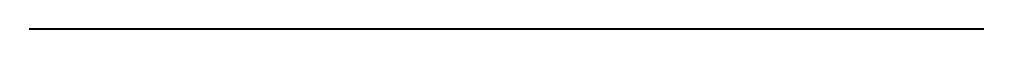
\begin{tikzpicture}
            \draw[thick, left color=gray, right color=white] (0,0) -- (\linewidth,0);
        \end{tikzpicture}
    \end{center}
}

\begin{center}
    \vspace*{1cm} % Use \vspace* for fixed positioning on the page
    {\Huge{\textbf{Lời mở đầu}}}    
\end{center}

\vspace{0.15cm} % Small space between title and line
\HRule % Minimalist thin line
\vspace{0.2cm} % Reduced space between line and content

Đồ án này là một phần của học phần \textit{Nhập môn lập trình kết nối vạn vật} - lớp 21KHDL, được tổ chức tại Khoa Công nghệ Thông tin, Trường Đại học Khoa học Tự nhiên, ĐHQG-HCM nhằm mục tiêu học tập, ứng dụng kiến thức IoT với tính chất là một đồ án phi thương mại. 


Em xin chân thành cảm ơn TS. Nguyễn Đức Hoàng Hạ, ThS. Đỗ Thị Thanh Hà, giảng viên Khoa Công nghệ Thông tin đã tận tình tư vấn, hỗ trợ về mặt kiến thức và định hướng, giúp cá nhân em hiểu rõ hơn về các nguyên lý và kỹ thuật cần thiết để hoàn thành đồ án này.
Đồng thời xin cảm ơn bạn Trần Lê Kim Ngân, sinh viên Khoa Điện tử Viễn thông, đã hỗ trợ nhiệt tình các linh kiện và vật liệu dựng mô hình cần thiết, góp phần quan trọng vào thành công của đồ án.


Sự hỗ trợ quý báu này là động lực quan trọng để bản thân em có thể hoàn thành dự án một cách tốt nhất. Mọi góp ý xin liên hệ qua email \href{mailto:thtam21@clc.fitus.edu.vn}{thtam21@clc.fitus.edu.vn}.\\[0.05cm]


\textit{Trân trọng,}


Trần Hiếu Tâm
\vspace{0.1cm} % Small space between title and line
\HRule % Minimalist thin line

\vfill

\end{titlepage}